% =====================================================================
% Guía del estudiante -- Geometría 11° -- Trimestre I
% María Mercedes Cantillo · Colegio San Alberto Magno
% ---------------------------------------------------------------------
% Plan: guia-periodo-I-hiperbola-navegacion.plan.md (y curriculo/plan-anual.md).
% Cada \tema tiene \label{tema:...} para que las clases lo citen con
% \refguia{tema:...}. No borrar el .aux de esta guía.
%
% Compilar:  latexmk -pdf guia-periodo-I-hiperbola-navegacion.tex
% =====================================================================
% BORRADOR: el plan del trimestre está pendiente de aprobación de la docente (generación rápida 2026-09-14).
\documentclass[11pt]{article}
\makeatletter\def\input@path{{../../../../plantillas/estilo/}}\makeatother
\usepackage{mmcantillo}

% ======================== DATOS DE LA GUÍA ============================
\tipodocumento{Guía del estudiante}
\asignatura{Geometría}
\titulo{Coordenadas, lugares geométricos y la hipérbola}
\grado{11°}
\periodo{I}
\hiloconductor{LORAN: encontrar un barco con dos hipérbolas}
% ======================================================================
% DBA: matematicas grado 11 · DBA 6 — Modela objetos geométricos en diversos sistemas
%      de coordenadas (cartesiano, polar, esférico) y realiza comparaciones y toma
%      decisiones con respecto a los modelos.
%      DBA 4 — Interpreta y diseña técnicas para hacer mediciones con niveles
%      crecientes de precisión (uso de diferentes instrumentos para la misma medición,
%      revisión de escalas y rangos de medida, estimaciones, verificaciones a través de
%      mediciones indirectas).

\begin{document}

\encabezado

% ---------------------------------------------------------------------
% 1. Frase introductoria
% ---------------------------------------------------------------------
% verificado: https://www.gutenberg.org/ebooks/26400 — La Géométrie (1637), libro I, primera frase: «Tous les problèmes de géométrie se peuvent facilement réduire à tels termes, qu'il n'est besoin par après que de connoître la longueur de quelques lignes droites pour les construire.»
\frase{Todos los problemas de geometría se pueden reducir fácilmente a tales
términos que después no hace falta conocer más que la longitud de algunas líneas
rectas para construirlos.}
{René Descartes, \emph{La geometría} (1637), libro I, trad. propia}

% ---------------------------------------------------------------------
% 2. Introducción
% ---------------------------------------------------------------------
\seccion{Introducción}

En la segunda semana del año quedó abierta una pregunta de investigación: ¿cómo
podía un barco en medio del océano, sin satélites, saber dónde estaba escuchando
señales de radio? La respuesta tiene nombre, \textbf{LORAN} (\emph{LOng RAnge
Navigation}, navegación de largo alcance), y una forma: la \textbf{hipérbola}. En
este trimestre vamos a construir, paso a paso, toda la geometría que hace falta para
entenderlo: el plano cartesiano como modelo del mapa, los lugares geométricos
(circunferencia, mediatriz e hipérbola) y el cálculo de una posición a partir de
diferencias de tiempo. Y como toda posición medida tiene un error, también
hablaremos de precisión.

Nuestro hilo conductor es la historia de LORAN: de una idea de 1940 a un sistema que
guió barcos y aviones durante casi setenta años, hasta que el GPS lo reemplazó. La
hipérbola la presentamos completa, desde su definición, porque la necesitamos para
LORAN; si ya la estudiaste, este tema te servirá de repaso.

\textbf{Al terminar este trimestre podrás:}
\begin{itemize}
  \item modelar un mapa con coordenadas cartesianas y calcular distancias y puntos medios;
  \item describir con ecuaciones la circunferencia, la mediatriz y la hipérbola como lugares geométricos;
  \item encontrar la ecuación de una hipérbola, sus vértices, focos y asíntotas;
  \item ubicar un punto como el cruce de dos hipérbolas y explicar la diferencia entre precisión y exactitud.
\end{itemize}

Este trimestre trabaja dos Derechos Básicos de Aprendizaje del Ministerio de
Educación Nacional~\cite{mendba}:

\begin{dba}[Grado 11 · DBA 6]
Modela objetos geométricos en diversos sistemas de coordenadas (cartesiano, polar,
esférico) y realiza comparaciones y toma decisiones con respecto a los modelos.
\end{dba}

\begin{dba}[Grado 11 · DBA 4]
Interpreta y diseña técnicas para hacer mediciones con niveles crecientes de
precisión (uso de diferentes instrumentos para la misma medición, revisión de
escalas y rangos de medida, estimaciones, verificaciones a través de mediciones
indirectas).
\end{dba}

% ---------------------------------------------------------------------
% 3. Marco teórico
% ---------------------------------------------------------------------
\seccion{Marco teórico}

\subsubsection*{Apolonio pone nombre a las cónicas}

Las curvas que se obtienen al cortar un cono con un plano fueron estudiadas por los
griegos durante siglos. Apolonio de Perga (c. 262--190 a.\,C.) escribió sobre ellas
los ocho libros de las \emph{Cónicas} y les dio los nombres que usamos todavía:
parábola, elipse e \textbf{hipérbola}~\cite{mactutorapolonio}. Siglos después, en
Alejandría, la matemática y filósofa Hipatia (c. 370--415) enseñaba la obra de los
griegos; una fuente bizantina tardía le atribuye un comentario a las \emph{Cónicas},
aunque los historiadores dudan de que lo haya escrito~\cite{mactutorhipatia}.

\subsubsection*{Descartes: la geometría con coordenadas}

En 1637, René Descartes publicó \emph{La geometría}, donde mostró que los problemas
de geometría se pueden traducir a relaciones entre longitudes, es decir, a
ecuaciones~\cite{descartes}. Esa idea es la base de la geometría analítica: un punto
es un par de números, una curva es una ecuación, y las propiedades de las figuras
se pueden calcular.

\subsubsection*{LORAN: una hipérbola para cada señal}

En octubre de 1940, el físico estadounidense Alfred Loomis propuso un sistema de
navegación por pulsos de radio basado en hipérbolas. El Laboratorio de Radiación del
MIT, creado ese mismo mes, lo desarrolló, aprovechando la experiencia del sistema
británico Gee, que también medía diferencias en el tiempo de llegada de señales. En
junio de 1942 ya transmitían las primeras estaciones, en Montauk Point (Nueva York) y
Fenwick Island (Delaware), y el 1 de enero de 1943 el sistema pasó a la
Armada. Su alcance era de unas 700 millas náuticas de día y hasta 1\,400 de noche, y
los errores de posición eran de cerca del 1~\% de la distancia a las
estaciones~\cite{merrill}. En los años setenta se reemplazó por LORAN-C, que daba
posiciones con errores de apenas cientos de pies~\cite{noaa}. Cuando el GPS se
volvió el sistema principal, la Guardia Costera de los Estados Unidos anunció el
apagado de LORAN-C a partir del 8 de febrero de 2010~\cite{fedreg}.

La idea es sencilla: dos estaciones emiten pulsos sincronizados; como las ondas de
radio viajan a la rapidez de la luz, $c = \num{299792458}$~m/s (un valor
exacto por definición~\cite{nist}), es decir, unos $300$~m por microsegundo, una
diferencia en el tiempo de llegada es una diferencia de distancias. Y el conjunto de
puntos cuya diferencia de distancias a dos puntos fijos es constante es una
hipérbola.

\subsubsection*{Gladys West: la forma de la Tierra para el GPS}

El GPS cambió las hipérbolas por esferas: el receptor calcula su distancia a varios
satélites. Pero para convertir esas distancias en una posición sobre el suelo hay
que conocer con mucha precisión la forma de la Tierra, que no es una esfera
perfecta. En el centro naval de Dahlgren (Virginia), la matemática \textbf{Gladys
West} programó durante años los cálculos de un modelo muy preciso de esa forma, el
geoide, que se usó en el sistema que llegó a ser el GPS. En 2018 fue incluida en el
Salón de la Fama de los pioneros espaciales y de misiles de la Fuerza Aérea de los
Estados Unidos~\cite{west}.

Las preguntas del Icfes se reproducen textualmente del cuadernillo
oficial~\cite{icfes2026}.

% ---------------------------------------------------------------------
% 4. Temas
% ---------------------------------------------------------------------
\tema{Coordenadas cartesianas}\label{tema:coordenadas}

\begin{hilo}
1942: Montauk Point y Fenwick Island, dos estaciones en la costa este de los
Estados Unidos. Para calcular dónde está un barco, lo primero es poner números a los
lugares: un origen, dos ejes y una unidad. El mapa se convierte en un plano cartesiano.
\end{hilo}

\begin{definicion}[Distancia y punto medio]
Para $A(x_1, y_1)$ y $B(x_2, y_2)$:
\[
  d(A, B) = \sqrt{(x_2 - x_1)^2 + (y_2 - y_1)^2}, \qquad
  M = \left(\frac{x_1 + x_2}{2}, \frac{y_1 + y_2}{2}\right).
\]
La fórmula de la distancia es el teorema de Pitágoras: las diferencias de
coordenadas son los catetos y el segmento $AB$ es la hipotenusa.
\end{definicion}

\begin{ejemplo}[Dos mapas, la misma distancia]
En un mapa con el origen en el puerto (unidades en km), una estación está en
$E(0, 0)$ y un barco en $B(30, 40)$: $d = \sqrt{30^2 + 40^2} = 50$~km. En otro mapa,
con el origen en un faro situado $20$~km al este y $10$~km al norte del puerto, las
coordenadas cambian (se resta $(20, 10)$): $E'(-20, -10)$ y $B'(10, 30)$. Pero la
distancia es la misma: $\sqrt{30^2 + 40^2} = 50$~km. Las coordenadas dependen del
sistema de referencia; las distancias y las formas, no.
\end{ejemplo}

\begin{aplicacion}[Coordenadas en el celular]
La aplicación de mapas de un celular guarda cada lugar como un par de números
(latitud y longitud). Para distancias cortas, como las de un barrio, se puede
trabajar como en un plano cartesiano y calcular distancias con Pitágoras; para
distancias entre ciudades hay que tener en cuenta que la Tierra es redonda (lo
veremos en el tercer trimestre).
\end{aplicacion}

\begin{preguntas}
% Ejercicio: medicion-11-005
\pregunta Calcula el perímetro del terreno de vértices $(0, 0)$, $(3, 0)$, $(5, 1)$,
$(6, 3)$, $(5, 5)$, $(2, 5)$ y $(0, 2)$ (en metros), en forma exacta y aproximado a
centésimas.
\espacio{3.5cm}
% Ejercicio: medicion-11-002
\Needspace{7\baselineskip}
\pregunta Calcula por triangulación el área del pentágono de vértices $(0, 0)$,
$(4, 0)$, $(5, 2)$, $(1, 4)$ y $(0, 2)$ (en centímetros), trazando las diagonales
desde el vértice $(0, 2)$.
\espacio{3cm}
% Ejercicio: medicion-11-001
\Needspace{8\baselineskip}
\pregunta En papel cuadriculado (cuadros de 1 cm) se dibuja el cuadrilátero de
vértices $A(0, 0)$, $B(5, 0)$, $C(4, 3)$ y $D(0, 1)$. Para hallar su área se traza la
diagonal $BD$, que lo divide en el triángulo rectángulo $ABD$ y el triángulo $BCD$;
en este último se midieron con regla la base $BD \approx \num{5,1}$ cm y la altura
sobre ella, $\approx \num{2,75}$ cm.
\begin{opciones}
  \item Calcula el área con esas medidas.
  \item Calcula el área exacta con las coordenadas.
  \item ¿Cuál es el error de la medición, en cm² y en porcentaje?
\end{opciones}
\espacio{3.5cm}
\end{preguntas}

\begin{resumen}
\begin{itemize}
  \item $d = \sqrt{(\Delta x)^2 + (\Delta y)^2}$ (Pitágoras) y $M$ = promedio de las coordenadas.
  \item Cambiar el origen cambia las coordenadas, pero no las distancias.
  \item Un cálculo con coordenadas exactas sirve para comprobar una medición con instrumentos.
\end{itemize}
\end{resumen}

% ---------------------------------------------------------------------
\tema{Lugares geométricos}\label{tema:lugares}

\begin{hilo}
Una estación emite un pulso y el barco lo recibe un tiempo $t$ después: está a una
distancia $c \cdot t$, pero ¿en qué dirección? Puede estar en cualquier punto de una
circunferencia. Y si el barco recibe al mismo tiempo los pulsos de dos estaciones
sincronizadas, está a igual distancia de las dos: sobre su mediatriz.
\end{hilo}

Un \textbf{lugar geométrico} es el conjunto de todos los puntos que cumplen una
condición. Traducir la condición a coordenadas da su ecuación.

\begin{definicion}[Circunferencia y mediatriz]
\textbf{Circunferencia} de centro $(h, k)$ y radio $r$: los puntos a distancia $r$
del centro,
\[ (x - h)^2 + (y - k)^2 = r^2. \]
\textbf{Mediatriz} del segmento $AB$: los puntos $P$ con $d(P, A) = d(P, B)$. Es la
recta perpendicular a $AB$ que pasa por su punto medio.
\end{definicion}

% Ejemplo resuelto: (x−3)² + (y+2)² − 25 = x² + y² − 6x + 4y − 12 (comprobado con SymPy)
\begin{ejemplo}[Completar cuadrados]
¿Qué figura es $x^2 + y^2 - 6x + 4y - 12 = 0$? Se agrupa y se completan cuadrados:
\[
  (x^2 - 6x + 9) + (y^2 + 4y + 4) = 12 + 9 + 4
  \;\Longrightarrow\; (x - 3)^2 + (y + 2)^2 = 25.
\]
Es la circunferencia de centro $(3, -2)$ y radio $5$.
\end{ejemplo}

\begin{aplicacion}[La cobertura de una antena]
Una antena de radio o de internet llega hasta cierta distancia: los lugares con
señal forman un círculo, y el borde de la cobertura es una circunferencia. Las
empresas de telecomunicaciones ubican sus antenas estudiando cómo se superponen esos
círculos, para que no queden zonas sin señal.
\end{aplicacion}

\begin{preguntas}
% Ejercicio: lugares-geometricos-11-003
\pregunta Una estación en el origen emite un pulso de radio que tarda
$200$~\unit{\micro\second} en llegar a un barco. Las ondas de radio viajan a unos
$\num{0,3}$~km/\unit{\micro\second}.
\begin{opciones}
  \item ¿A qué distancia está el barco?
  \item ¿Dónde puede estar? Escribe la ecuación.
  \item ¿Por qué una sola estación no basta para saber la posición?
\end{opciones}
\espacio{3cm}
% Ejercicio: lugares-geometricos-11-004
\pregunta Dos estaciones están en $A(0, 0)$ y $B(8, 4)$. Halla la ecuación de la
mediatriz de $AB$ (los puntos a igual distancia de las dos) y comprueba que $(5, 0)$
está a igual distancia de $A$ y de $B$.
\espacio{3cm}
% Ejercicio: icfes-cuadernillo-2026-037
\Needspace{11\baselineskip}
\pregunta (Icfes, Saber 11.º, 2026, pregunta 37.) Sobre una circunferencia de centro
$O$ se localizan dos puntos $P$ y $P'$ diferentes. De las siguientes, ¿cuál figura NO
puede resultar al unir entre sí los tres puntos $P$, $P'$ y $O$?
\begin{opciones*}(2)
  \item Un triángulo isósceles.
  \item Un radio de la circunferencia.
  \item Un triángulo equilátero.
  \item Un diámetro de la circunferencia.
\end{opciones*}
Justifica tu respuesta.
\renglones{2}
\end{preguntas}

\begin{resumen}
\begin{itemize}
  \item Circunferencia: distancia constante a un punto; $(x - h)^2 + (y - k)^2 = r^2$.
  \item Mediatriz: igual distancia a dos puntos; es una recta.
  \item Para reconocer una circunferencia en la forma general, se completan cuadrados.
\end{itemize}
\end{resumen}

% ---------------------------------------------------------------------
\tema{La hipérbola}\label{tema:hiperbola}

\begin{hilo}
Lo normal es que los dos pulsos \emph{no} lleguen al mismo tiempo. Si el de la
estación $B$ llega $400$ microsegundos antes que el de $A$, el barco está unos
$120$~km más cerca de $B$ que de $A$. ¿Qué forma tiene el conjunto de todos esos
puntos? Esa es la curva que Loomis vio en su propuesta de 1940.
\end{hilo}

\begin{definicion}[Hipérbola]
Dados dos puntos $F_1$ y $F_2$ (los \textbf{focos}), una \textbf{hipérbola} es el
conjunto de puntos $P$ cuya diferencia de distancias a los focos es constante:
\[ \abs{d(P, F_1) - d(P, F_2)} = 2a, \qquad \text{con } 0 < 2a < d(F_1, F_2). \]
\end{definicion}

\begin{teorema}[Ecuación canónica]
Si los focos son $F_1(-c, 0)$ y $F_2(c, 0)$, la hipérbola es
\[
  \frac{x^2}{a^2} - \frac{y^2}{b^2} = 1, \qquad \text{donde } b^2 = c^2 - a^2
  \;\;(\text{es decir, } c^2 = a^2 + b^2).
\]
Sus \textbf{vértices} son $(\pm a, 0)$, sus \textbf{asíntotas} son las rectas
$y = \pm \frac{b}{a}\,x$, y tiene dos \textbf{ramas}: la de la derecha, más cerca de
$F_2$, y la de la izquierda, más cerca de $F_1$.
\end{teorema}

\emph{De dónde sale.} Se escribe la condición con la fórmula de la distancia,
$\sqrt{(x + c)^2 + y^2} - \sqrt{(x - c)^2 + y^2} = \pm 2a$, se aísla una raíz, se
eleva al cuadrado dos veces y se simplifica; con $b^2 = c^2 - a^2$ queda la ecuación
canónica. La condición $2a < 2c$ es necesaria por la desigualdad triangular: en el
triángulo $PF_1F_2$, la diferencia de dos lados es menor que el tercero.

% Ejemplo resuelto (no es ejercicio): comprobado con SymPy — PF1 = 34/3, PF2 = 16/3, diferencia 6; b² = 25 − 9 = 16
\begin{ejemplo}[Del foco a la ecuación]
Los focos son $F_1(-5, 0)$ y $F_2(5, 0)$ y la diferencia de distancias es $6$.
Entonces $2a = 6$, $a = 3$, $c = 5$ y $b^2 = 25 - 9 = 16$:
\[ \frac{x^2}{9} - \frac{y^2}{16} = 1. \]
Vértices $(\pm 3, 0)$; asíntotas $y = \pm \frac{4}{3}x$. Comprobación con el punto
$P\left(5, \frac{16}{3}\right)$: $PF_1 = \frac{34}{3}$, $PF_2 = \frac{16}{3}$ y
$\frac{34}{3} - \frac{16}{3} = 6$.
\begin{center}
\begin{tikzpicture}
\begin{axis}[mmc, xmin=-8, xmax=8, ymin=-7, ymax=7, axis equal image,
             xtick={-3,3}, ytick={-4,4},
             width=0.55\linewidth]
  \addplot+[domain=-1.6:1.6, samples=60, mark=none] ({3*cosh(x)}, {4*sinh(x)});
  \addplot+[domain=-1.6:1.6, samples=60, mark=none, solid] ({-3*cosh(x)}, {4*sinh(x)});
  \addplot[thin, dashed, domain=-8:8] {4*x/3};
  \addplot[thin, dashed, domain=-8:8] {-4*x/3};
  \addplot[only marks, mark=*, mark size=1.8pt] coordinates {(-5,0) (5,0)};
  \addplot[only marks, mark=o, mark size=1.8pt] coordinates {(-3,0) (3,0)};
  \node[below] at (axis cs:-5,0) {\small $F_1$};
  \node[below] at (axis cs:5,0) {\small $F_2$};
\end{axis}
\end{tikzpicture}

{\small Las dos ramas de $\frac{x^2}{9} - \frac{y^2}{16} = 1$, sus focos (puntos
negros), vértices (puntos blancos) y asíntotas (a trazos).}
\end{center}
\end{ejemplo}

\emph{Para construirla con hilo:} se fija un extremo de una regla en $F_1$ y se
ata un hilo del otro extremo de la regla a $F_2$, con el hilo $2a$ más corto que la
regla; al girar la regla manteniendo el hilo tenso con un lápiz contra la regla, el
lápiz dibuja una rama. (En GeoGebra: el comando \texttt{Hipérbola(F1, F2, a)}.)

\begin{aplicacion}[¿De dónde viene un sonido?]
Si un mismo sonido llega a dos micrófonos en tiempos distintos, la diferencia de
tiempos multiplicada por la rapidez del sonido da la diferencia de distancias: la
fuente está sobre una hipérbola cuyos focos son los micrófonos. Con varios
micrófonos, las hipérbolas se cortan en el punto de origen del sonido. Es el mismo
principio de LORAN, con sonido en lugar de radio.
\end{aplicacion}

\begin{preguntas}
% Ejercicio: hiperbola-11-002
\pregunta Para la hipérbola $\frac{x^2}{16} - \frac{y^2}{9} = 1$ halla $a$, $b$, $c$,
los vértices, los focos y las asíntotas. Dibújala en tu cuaderno.
\espacio{4cm}
% Ejercicio: hiperbola-11-004
\pregunta Laura tiene la hipérbola $\frac{x^2}{16} - \frac{y^2}{9} = 1$ y calcula sus
focos así: «$c^2 = a^2 - b^2 = 16 - 9 = 7$, así que los focos son
$(\pm\sqrt{7}, 0)$». ¿Cuál es el error? Muestra que el punto $(4, 0)$ no cumple la
definición con esos focos.
\espacio{3.5cm}
\end{preguntas}

\begin{resumen}
\begin{itemize}
  \item Hipérbola: diferencia de distancias a los focos constante, igual a $2a$.
  \item Centro en el origen y focos en el eje $x$: $\frac{x^2}{a^2} - \frac{y^2}{b^2} = 1$, con $c^2 = a^2 + b^2$.
  \item Vértices $(\pm a, 0)$, focos $(\pm c, 0)$, asíntotas $y = \pm \frac{b}{a}x$.
\end{itemize}
\end{resumen}

% ---------------------------------------------------------------------
\tema{Navegación hiperbólica}\label{tema:navegacion}

\begin{hilo}
Una hipérbola dice «estás en algún punto de esta curva», pero no en cuál. Por eso
LORAN usaba cadenas de estaciones: un segundo par da otra hipérbola, y el barco está
donde las dos se cruzan. Los navegantes tenían cartas con las hipérbolas ya
dibujadas y solo buscaban el cruce de las dos que indicaba su receptor.
\end{hilo}

\begin{teorema}[De tiempos a distancias]
Si las señales viajan con rapidez $v$ y un receptor mide una diferencia de tiempos
$\Delta t$ entre los pulsos de dos estaciones sincronizadas, la diferencia de sus
distancias a las estaciones es
\[ \Delta d = v \cdot \Delta t \qquad (\text{para ondas de radio, } v \approx \num{0,3}~\text{km}/\unit{\micro\second}). \]
El barco está sobre la hipérbola con focos en las estaciones y $2a = \Delta d$, en la
rama de la estación cuyo pulso llegó primero. Esa rama es una \textbf{línea de posición}.
\end{teorema}

% Ejemplo resuelto (no es ejercicio): comprobado con SymPy — 0,3·400 = 120; b² = 300² − 60² = 86 400
\begin{ejemplo}[Una línea de posición]
Dos estaciones $A(-300, 0)$ y $B(300, 0)$ (en km) emiten pulsos al mismo tiempo, y un
barco recibe el de $B$ $400$~\unit{\micro\second} antes que el de $A$. Entonces
$d_A - d_B = \num{0,3} \cdot 400 = 120$~km, así que $2a = 120$, $a = 60$, $c = 300$ y
$b^2 = 90\,000 - 3\,600 = 86\,400$. El barco está sobre
\[ \frac{x^2}{3\,600} - \frac{y^2}{86\,400} = 1, \]
en la rama de la derecha ($x > 0$), la más cercana a $B$.
\end{ejemplo}

\begin{center}
\begin{tikzpicture}
\begin{axis}[mmc, xmin=0, xmax=8, ymin=0, ymax=8, axis equal image,
             xtick={5}, ytick={5}, width=0.5\linewidth]
  \addplot+[domain=0:1.4, samples=50, mark=none] ({3*cosh(x)}, {4*sinh(x)});
  \addplot+[domain=0:1.4, samples=50, mark=none] ({4*sinh(x)}, {3*cosh(x)});
  \addplot[only marks, mark=*, mark size=1.8pt] coordinates {(5,0) (0,5)};
  \addplot[only marks, mark=square*, mark size=2pt] coordinates {(4.5356,4.5356)};
  \node[above left] at (axis cs:5,0) {\small $F_2$};
  \node[above right] at (axis cs:0,5) {\small $F_4$};
  \node[right] at (axis cs:4.6,4.3) {\small barco};
\end{axis}
\end{tikzpicture}

{\small Dos líneas de posición (ramas de $\frac{x^2}{9} - \frac{y^2}{16} = 1$ y de
$\frac{y^2}{9} - \frac{x^2}{16} = 1$, en unidades de 100~km) y su cruce.}
\end{center}

\subsubsection*{Precisión y exactitud}

Como la señal recorre unos $300$~m en un microsegundo, un error de $1$~\unit{\micro\second}
en el reloj del receptor es un error de $300$~m en la diferencia de distancias; para
errores de decenas de metros hay que medir tiempos con precisión de décimas de
microsegundo. Además hay que distinguir dos cosas. Una medición es \textbf{precisa}
si al repetirla se obtienen valores muy parecidos entre sí, y es \textbf{exacta} si
esos valores están cerca del valor real. Un receptor con un retraso fijo puede dar
medidas muy precisas\ldots\ y todas equivocadas.

\begin{aplicacion}[Del LORAN al GPS]
El GPS usa la misma idea con otra geometría: en lugar de diferencias de distancias a
estaciones en tierra (hipérbolas), el receptor calcula sus distancias a varios
satélites (esferas) y busca el punto común. Su precisión depende de relojes atómicos
en los satélites y de un modelo muy preciso de la forma de la Tierra, como el que
calculó Gladys West.
\end{aplicacion}

\begin{preguntas}
% Ejercicio: navegacion-11-003
\pregunta Unidades: $100$~km. Un par de estaciones en $(\pm 5, 0)$ ubica al barco
sobre $\frac{x^2}{9} - \frac{y^2}{16} = 1$, rama derecha; otro par en $(0, \pm 5)$ lo
ubica sobre $\frac{y^2}{9} - \frac{x^2}{16} = 1$, rama superior. Halla la posición
del barco.
\espacio{4.5cm}
% Ejercicio: navegacion-11-005
\pregunta Un receptor mide cuatro veces la diferencia de tiempos para el mismo
barco quieto: $\num{400,2}$; $\num{399,8}$; $\num{400,1}$ y $\num{399,9}$~\unit{\micro\second}.
\begin{opciones}
  \item Halla el promedio y la diferencia de distancias.
  \item ¿Cuánto varían las distancias entre la medida mayor y la menor?
  \item Después se descubre que el receptor tiene un retraso fijo de
        $5$~\unit{\micro\second} en todas sus medidas. ¿Las medidas eran precisas?
        ¿Eran exactas? ¿Cuánto error produce el retraso?
\end{opciones}
\espacio{4cm}
\end{preguntas}

\begin{resumen}
\begin{itemize}
  \item $\Delta d = v\,\Delta t$: una diferencia de tiempos es una diferencia de distancias.
  \item Un par de estaciones da una hipérbola (línea de posición); dos pares, un cruce: la posición.
  \item Precisión: medidas parecidas entre sí; exactitud: cercanas al valor real.
\end{itemize}
\end{resumen}

% ---------------------------------------------------------------------
% 5. Prepárate para Saber 11
% ---------------------------------------------------------------------
\seccion{Prepárate para Saber 11}

\begin{instrucciones}
Preguntas de selección múltiple con única respuesta, como las de la prueba Saber 11.
Las tres son del cuadernillo oficial de preguntas del Icfes~\cite{icfes2026}
(preguntas 32, 50 y 17) y se reproducen sin cambios.
\end{instrucciones}

\begin{preguntas}
% Ejercicio: icfes-cuadernillo-2026-032
\pregunta Un trapecio isósceles es un trapecio cuyos lados no paralelos son
congruentes. En un plano cartesiano se dibuja un trapecio isósceles de modo que el
eje $y$ divide al trapecio en dos figuras iguales. Si las coordenadas de dos de los
vértices del trapecio son $(-4, 2)$ y $(-2, 8)$, ¿cuáles son las coordenadas de los
otros dos vértices?
\begin{opciones*}(2)
  \item $(8, 2)$ y $(2, 4)$.
  \item $(2, 8)$ y $(4, 2)$.
  \item $(-2, -4)$ y $(-8, -2)$.
  \item $(-4, -2)$ y $(-2, -8)$.
\end{opciones*}
% Ejercicio: icfes-cuadernillo-2026-050
\Needspace{18\baselineskip}
\pregunta Alfonso tiene tres empaques para almacenar dulces. Los empaques y las
medidas de estos se muestran en la figura.

\begin{center}
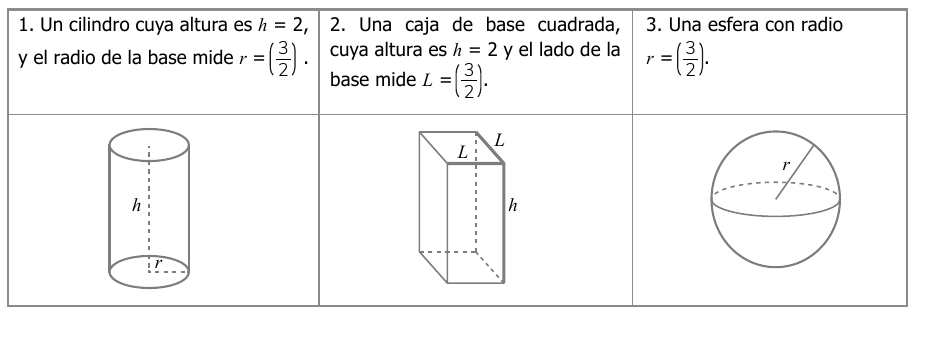
\includegraphics[width=0.85\linewidth]{figuras/icfes-2026-p50.png}
\end{center}

¿Cuál de las siguientes afirmaciones es verdadera respecto al volumen de los tres
empaques?
\begin{opciones}
  \item El volumen del cilindro es mayor que el volumen de la caja; además, el
        volumen de la esfera es igual que el volumen del cilindro.
  \item El volumen del cilindro es igual que el volumen de la caja; además, el
        volumen de la esfera es mayor que el volumen del cilindro.
  \item El volumen del cilindro es menor que el volumen de la caja; además, el
        volumen de la esfera es igual que el volumen del cilindro.
  \item El volumen del cilindro es mayor que el volumen de la caja; además, el
        volumen de la esfera es mayor que el volumen del cilindro.
\end{opciones}
% Ejercicio: icfes-cuadernillo-2026-017
\Needspace{12\baselineskip}
\pregunta La longitud de las aristas de la caja de la figura son $l$, $a$ y $h$.

\begin{center}
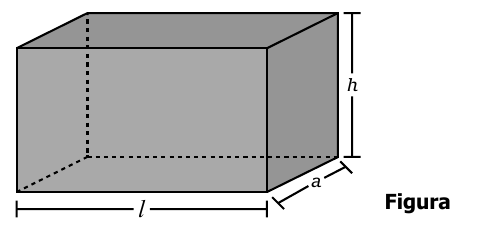
\includegraphics[width=0.45\linewidth]{figuras/icfes-2026-p17.png}
\end{center}

¿Cuál de las siguientes expresiones determina la longitud total de las aristas de
la caja?
\begin{opciones*}(4)
  \item $lah$
  \item $4lah$
  \item $l+a+h$
  \item $4l + 4a + 4h$
\end{opciones*}
\end{preguntas}

% ---------------------------------------------------------------------
% 6. Cierre del hilo conductor
% ---------------------------------------------------------------------
\seccion{Cierre: de las hipérbolas a las esferas}

Apolonio nombró la hipérbola hace más de dos mil años sin imaginar que serviría para
navegar. Descartes le dio una ecuación, Loomis la convirtió en una línea de
posición, y durante casi setenta años miles de barcos y aviones encontraron su
camino cortando dos de ellas. Hoy el GPS hace lo mismo con esferas, gracias a
modelos de la Tierra como el de Gladys West. En el segundo trimestre seguiremos con
la medición: precisión, mediciones indirectas, áreas y volúmenes, y los sistemas de
coordenadas polares y tridimensionales que evalúa la prueba Saber 11.

% ---------------------------------------------------------------------
% 7. Evaluación (secciones institucionales)
% ---------------------------------------------------------------------
\matrizevaluacion
  {Explica la circunferencia, la mediatriz y la hipérbola como lugares geométricos y
   relaciona sus ecuaciones con sus elementos.}
  {Calcula distancias, puntos medios y ecuaciones de lugares geométricos; ubica un
   punto como cruce de dos hipérbolas y estima la precisión de una posición medida.}
  {Justifica sus procedimientos, revisa sus errores y distingue entre una medida
   precisa y una exacta.}
  {Trabaja en equipo en la investigación y la socialización, y reconoce el aporte de
   mujeres y hombres de distintas épocas a la geometría y la navegación.}

\autoevaluacion

\seguimientodocente

% ---------------------------------------------------------------------
% 8. Referencias
% ---------------------------------------------------------------------
\begin{referencias}
% verificado: https://www.gutenberg.org/ebooks/26400 — La Géométrie (1637), texto francés completo (Project Gutenberg)
\bibitem{descartes} Descartes, R. (1637). \emph{La Géométrie}. Apéndice del
  \emph{Discours de la méthode}. Leiden: Ian Maire.
% verificado: https://www.federalregister.gov/documents/2010/01/07/2010-83/terminate-long-range-aids-to-navigation-loran-c-signal — 75 FR 998, 7 ene. 2010; terminación a partir del 8 feb. 2010
\bibitem{fedreg} Guardia Costera de los Estados Unidos (2010, 7 de enero). Terminate
  Long Range Aids to Navigation (Loran-C) Signal. \emph{Federal Register}, 75, 998.
% verificado: recursos/matematicas/icfes/09-Marzo_Cuadernillo-de-Preguntas-Matematicas-Saber-11-2026.pdf (archivo local) — Icfes, marzo de 2026
\bibitem{icfes2026} Icfes (2026). \emph{Cuadernillo de preguntas Saber 11.º: prueba de
  Matemáticas}. Bogotá: Instituto Colombiano para la Evaluación de la Educación.
% verificado: https://archive.navalsubleague.org/2006/loran-showing-the-way-long-range-navigation-land-sea-air-part-i-1940-1942 — The Submarine Review, enero de 2006
\bibitem{merrill} Merrill, J. (2006, enero). Loran showing the way: long range
  navigation (land, sea, air), Part I, 1940--1942. \emph{The Submarine Review}.
% verificado: https://gblumen.mineducacion.gov.co/cgi-bin/koha/opac-detail.pl?biblionumber=4785 — MEN 2016
\bibitem{mendba} Ministerio de Educación Nacional (2016). \emph{Derechos Básicos de
  Aprendizaje V.2: Matemáticas}. Bogotá: MEN.
% verificado: https://physics.nist.gov/cgi-bin/cuu/Value?c — 299 792 458 m/s (exacta)
\bibitem{nist} National Institute of Standards and Technology (s.\,f.). \emph{Speed of
  light in vacuum}. CODATA Internationally Recommended Values of the Fundamental
  Physical Constants.
% verificado: https://nauticalcharts.noaa.gov/updates/navigating-waters-before-gps-why-some-mariners-still-refer-to-loran-c/ — LORAN-C: posiciones «within hundreds of feet»; apagado en 2010
\bibitem{noaa} NOAA, Office of Coast Survey (s.\,f.). \emph{Navigating waters before
  GPS: why some mariners still refer to Loran-C}.
% verificado: https://mathshistory.st-andrews.ac.uk/Biographies/Apollonius/ — c. 262–190 a. C.; Conics en 8 libros; introdujo parábola, elipse, hipérbola
\bibitem{mactutorapolonio} O'Connor, J. J. y Robertson, E. F. (1999). \emph{Apollonius
  of Perga}. MacTutor History of Mathematics, University of St Andrews.
% verificado: https://mathshistory.st-andrews.ac.uk/Biographies/Hypatia/ — c. 370–415; la Suda le atribuye comentarios a las Cónicas; los historiadores lo dudan
\bibitem{mactutorhipatia} O'Connor, J. J. y Robertson, E. F. (1999). \emph{Hypatia of
  Alexandria}. MacTutor History of Mathematics, University of St Andrews.
% verificado: https://www.britannica.com/biography/Gladys-West — Dahlgren; modelo geodésico para el GPS; Salón de la Fama (6 dic. 2018)
\bibitem{west} Encyclopaedia Britannica (s.\,f.). \emph{Gladys West}.
\end{referencias}

\end{document}
